% This is the Latex template for my future homework write-ups
% A basic form of Latex command: '/command name[argu, argu]{argu*}' as below:
\documentclass[12pt, letterpaper]{article} % use 'tab' to complete 
% which means this document is an article with 12pt (font size) and letterpaper (paper type)


% ======================================================
% This is the preamble section for loading packages, a basic form looks like: 
% /usepackage{filename} the package name is the .sty file.  Let's load some 
% packages (Latex will complain if the .sty file is not in PWD):
% ======================================================
\usepackage{indentfirst} % indent the 1st line of the 1st paragraph, using \noindent to cancel
\usepackage{graphicx} % for using graphics


% ============================================================================
% These are basic settings for making title and content
% ============================================================================
% Now, we start the work by entering the document with:
\begin{document}  % always remember 'begin - end' pairs
% Basic settings for the title page
\title{\LaTeX: Phys 5391 Assignment 3} % title name
\author{Yu Hong\\Space Physics Group} % double-slash for new line
\date{October 12, 2020}  % or the \today command to insert today's date.
% Now setting the format of the article
\maketitle % make a title based on  the info above


% ============================================================================
% This Section is used for demonstrating some basic command of controlling Figures
% ============================================================================
% Package 'graphicx' is needed: already loaded
\graphicspath{ {./images/} } % Added the Figure path, or you can put it directly the same path with this code
\textbf{Figure 1} shows the temporal variation of IMF B$_y$ and B$_z$ (top panel), solar wind V$_x$ (2nd panel), density (3rd panel) and temperature (4th panel) as well as the geomagnetic field D$_{ST}$ index (5th panel) of July 15, 2000.

As mentioned in class, IMF represents the solar wind magnetic field measured at L1 point, while D$_{ST}$  indicates the geomagnetic field disturb during magnetospheric activity period. When B$_z$ turns to strong negatives at 17:30 UT, the D$_{ST}$  index reaches extreme big negative values with minimum around -300 nT, forming the storm. To clarify, we separate the time into 3 periods as indicated by the two vertical black dashed lines. 

\textbf{Period 1}: Before 14:00 UT, both the arriving solar wind and geomagnetic field are pretty quiet with very small variations. 

\textbf{Period 2}: At around 14:00 UT, a group of high-speed (~1000 km/s), hot and dense solar wind plasma with positive B$_y$ and B$_z$ (~20 nT) arrived at L1 point. At the same time, D$_{ST}$  index also changes with a positive increase up to 10 nT. The geomagnetic field can be compressed due to the high-speed V$_x$, leading to the increase of background positive (northward) geomagnetic field, thus the D$_{ST}$  index is reversed to a positive value. After this, although B$_z$ changes with time, the time period is not long enough to form a big geomagnetic field disturb.

\textbf{Period 3}: At around 17:30 UT, B$_z$ turns to big negative values, this is the switch of the well-known phenomenon “magnetic field reconnection”. During storm period, when magnetic reconnection happens in the Earth’s magnetosphere tail, the accelerated particle flow moves towards the Earth and forms a westward current with the effect of the geomagnetic field. The corresponding magnetic field due to the westward current is southward (negative), this is the D$_{ST}$  variation. Meanwhile, solar wind V$_x$ (negative means towards the Earth) also boosts this process. Since big V$_x$ means big kinetic energy (the density also increased as shown in the 3rd panel), this will accelerate the interaction with the geomagnetic field. 

In general, the IMF B$_z$ component is closely related to D$_{ST}$  index. When B$_z$ is continuously negative enough, a large negative D$_{ST}$  will be found. In addition, solar wind V$_x$ also enhances the interaction between the IMF and geomagnetic field. 

\begin{figure}[!t] % !b for bottom, t for top; ! for good position
\begin{center} % put the figure in the center 
  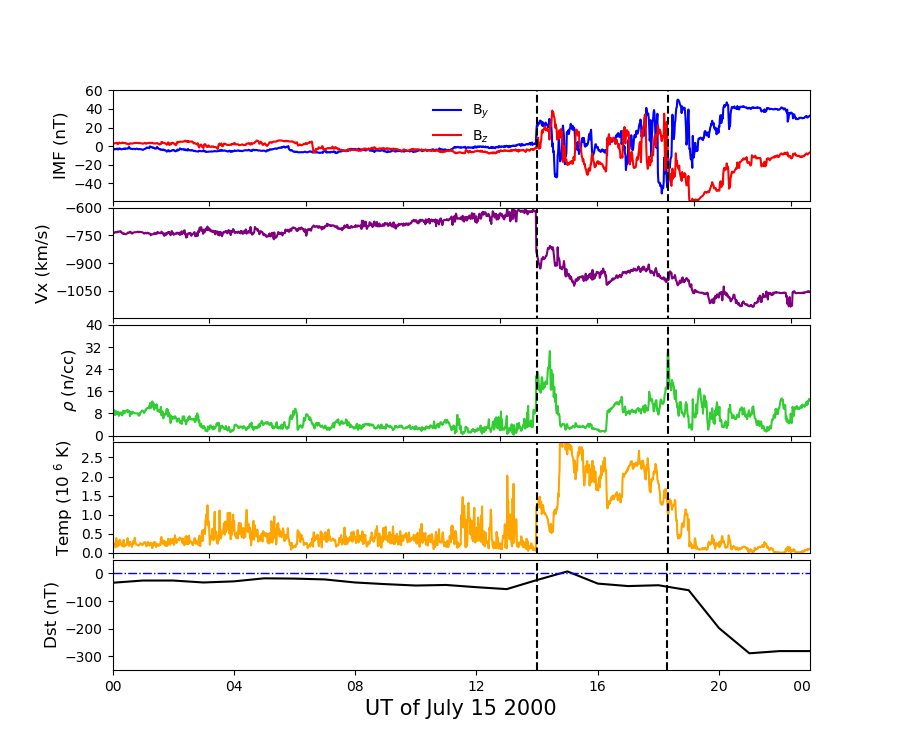
\includegraphics[width=13cm,height=13cm]{imf_dst.png} % changing figure size and rotate: scale=1.2, angle=45
  \caption{IMF and Dst of July 15, 2000} % This figure is in the same path as the code
  \label{png:imf_dst} % label the figure with the unique name "rick"
\end{center} % end the environment {center}
\end{figure} % end the environment {figure}



% End the document environment.  This is the last line for coding
\end{document}










